% -*- coding: utf-8 -*-
%-------------------------designed by zcf--------------
\documentclass[UTF8,a4paper,10pt]{ctexart}
\usepackage[left=3.17cm, right=3.17cm, top=2.74cm, bottom=2.74cm]{geometry}
\usepackage{amsmath}
\usepackage{graphicx,subfig}
\usepackage{float}
\usepackage{cite}
\usepackage{caption}
\usepackage{enumerate}
\usepackage{booktabs} %表格
\usepackage{multirow}
\newcommand{\tabincell}[2]{\begin{tabular}{@{}#1@{}}#2\end{tabular}}  %表格强制换行
%-------------------------字体设置--------------
% \usepackage{times} 
\usepackage{ctex}
\setCJKmainfont[ItalicFont=Noto Sans CJK SC Bold, BoldFont=Noto Serif CJK SC Black]{Noto Serif CJK SC}
\newcommand{\yihao}{\fontsize{26pt}{36pt}\selectfont}           % 一号, 1.4 倍行距
\newcommand{\erhao}{\fontsize{22pt}{28pt}\selectfont}          % 二号, 1.25倍行距
\newcommand{\xiaoer}{\fontsize{18pt}{18pt}\selectfont}          % 小二, 单倍行距
\newcommand{\sanhao}{\fontsize{16pt}{24pt}\selectfont}  %三号字
\newcommand{\xiaosan}{\fontsize{15pt}{22pt}\selectfont}        % 小三, 1.5倍行距
\newcommand{\sihao}{\fontsize{14pt}{21pt}\selectfont}            % 四号, 1.5 倍行距
\newcommand{\banxiaosi}{\fontsize{13pt}{19.5pt}\selectfont}    % 半小四, 1.5倍行距
\newcommand{\xiaosi}{\fontsize{12pt}{18pt}\selectfont}            % 小四, 1.5倍行距
\newcommand{\dawuhao}{\fontsize{11pt}{11pt}\selectfont}       % 大五号, 单倍行距
\newcommand{\wuhao}{\fontsize{10.5pt}{15.75pt}\selectfont}    % 五号, 单倍行距
%-------------------------章节名----------------
\usepackage{ctexcap} 
\CTEXsetup[name={,、},number={ \chinese{section}}]{section}
\CTEXsetup[name={(,)},number={\chinese{subsection}}]{subsection}
\CTEXsetup[name={,.},number={\arabic{subsubsection}}]{subsubsection}
%-------------------------页眉页脚--------------
\usepackage{fancyhdr}
\pagestyle{fancy}
\lhead{\kaishu \leftmark}
% \chead{}
\rhead{\kaishu 计算机网络第一次实验}%加粗\bfseries 
\lfoot{}
\cfoot{\thepage}
\rfoot{}
\renewcommand{\headrulewidth}{0.1pt}  
\renewcommand{\footrulewidth}{0pt}%去掉横线
\newcommand{\HRule}{\rule{\linewidth}{0.5mm}}%标题横线
\newcommand{\HRulegrossa}{\rule{\linewidth}{1.2mm}}
%-----------------------伪代码------------------
\usepackage{algorithm}  
\usepackage{algorithmicx}  
\usepackage{algpseudocode}  
\floatname{algorithm}{Algorithm}  
\renewcommand{\algorithmicrequire}{\textbf{Input:}}  
\renewcommand{\algorithmicensure}{\textbf{Output:}} 
\usepackage{lipsum}  
\makeatletter
\newenvironment{breakablealgorithm}
  {% \begin{breakablealgorithm}
  \begin{center}
     \refstepcounter{algorithm}% New algorithm
     \hrule height.8pt depth0pt \kern2pt% \@fs@pre for \@fs@ruled
     \renewcommand{\caption}[2][\relax]{% Make a new \caption
      {\raggedright\textbf{\ALG@name~\thealgorithm} ##2\par}%
      \ifx\relax##1\relax % #1 is \relax
         \addcontentsline{loa}{algorithm}{\protect\numberline{\thealgorithm}##2}%
      \else % #1 is not \relax
         \addcontentsline{loa}{algorithm}{\protect\numberline{\thealgorithm}##1}%
      \fi
      \kern2pt\hrule\kern2pt
     }
  }{% \end{breakablealgorithm}
     \kern2pt\hrule\relax% \@fs@post for \@fs@ruled
  \end{center}
  }
\makeatother
%------------------------代码-------------------
\usepackage{xcolor} 
\usepackage{listings} 
\lstset{ 
breaklines,%自动换行
basicstyle=\small,
escapeinside=``,
keywordstyle=\color{ blue!70} \bfseries,
commentstyle=\color{red!50!green!50!blue!50},% 
stringstyle=\ttfamily,% 
extendedchars=false,% 
linewidth=\textwidth,% 
numbers=left,% 
numberstyle=\tiny \color{blue!50},% 
frame=trbl% 
rulesepcolor= \color{ red!20!green!20!blue!20} 
}
%------------超链接----------
\usepackage[colorlinks,linkcolor=black,anchorcolor=blue]{hyperref}
%------------------------TODO-------------------
\usepackage{enumitem,amssymb}
\newlist{todolist}{itemize}{2}
\setlist[todolist]{label=$\square$}
% for check symbol 
\usepackage{pifont}
\newcommand{\cmark}{\ding{51}}%
\newcommand{\xmark}{\ding{55}}%
\newcommand{\done}{\rlap{$\square$}{\raisebox{2pt}{\large\hspace{1pt}\cmark}}\hspace{-2.5pt}}
\newcommand{\wontfix}{\rlap{$\square$}{\large\hspace{1pt}\xmark}}
%------------------------水印-------------------
\usepackage{tikz}
\usepackage{xcolor}
\usepackage{eso-pic}

\newcommand{\watermark}[3]{\AddToShipoutPictureBG{
\parbox[b][\paperheight]{\paperwidth}{
\vfill%
\centering%
\tikz[remember picture, overlay]%
  \node [rotate = #1, scale = #2] at (current page.center)%
    {\textcolor{gray!80!cyan!30!magenta!30}{#3}};
\vfill}}}



%———————————————————————————————————————————正文———————————————————————————————————————————————
%----------------------------------------------
\begin{document}
\begin{titlepage}
    \begin{center}
    
\includegraphics[width=0.8\textwidth]{NKU.png}\\[1cm]    
    \textsc{\Huge \kaishu{\textbf{南\ \ \ \ \ \ 开\ \ \ \ \ \ 大\ \ \ \ \ \ 学}} }\\[0.9cm]
    \textsc{\huge \kaishu{\textbf{网\ \ 络\ \ 空\ \ 间\ \ 安\ \ 全\ \ 学\ \ 院}}}\\[0.5cm]
    \textsc{\Large \textbf{计算机网络实验3-3}}\\[0.8cm]
    \HRule \\[0.9cm]
    { \LARGE \bfseries 基于UDP服务设计可靠传输协议并编程实现}\\[0.4cm]
    \HRule \\[2.0cm]
    \centering
    \textsc{\LARGE \kaishu{马世骐\ \ 6016252 }}\\[0.5cm]
    \textsc{\LARGE \kaishu{年级\ :\ 2020级}}\\[0.5cm]
    \textsc{\LARGE \kaishu{专业\ :\ 经济伯苓班}}\\[0.5cm]
    \textsc{\LARGE \kaishu{指导教师\ :\ 张建忠、徐敬东}}\\[0.5cm]
    \vfill
    {\Large \today}
    \end{center}
\end{titlepage}
%-------------摘------要--------------
\newpage
\thispagestyle{empty}
%----------------------------------------------------------------
\tableofcontents
%----------------------------------------------------------------
\newpage
\watermark{60}{10}{NKU}
\setcounter{page}{1}
%----------------------------------------------------------------
\section{实验基本描述}
%——————————————————————————————————————
在实验3-2的基础上实现了拥塞控制。

%----------------------------------------------------------------
\section{实验具体工作}
%——————————————————————————————————————
\begin{enumerate}
  \item 在3-2的基础上,增加流量控制功能
  \item 采用RENO算法
  \item 使用多线程编程
  \item 可以扫描文件夹下的文件,为文件传输和验证提供方便
\end{enumerate}
\section{协议设计(与之前实验相同)}
\subsubsection{报文格式}
\begin{figure}[H]
    \centering
    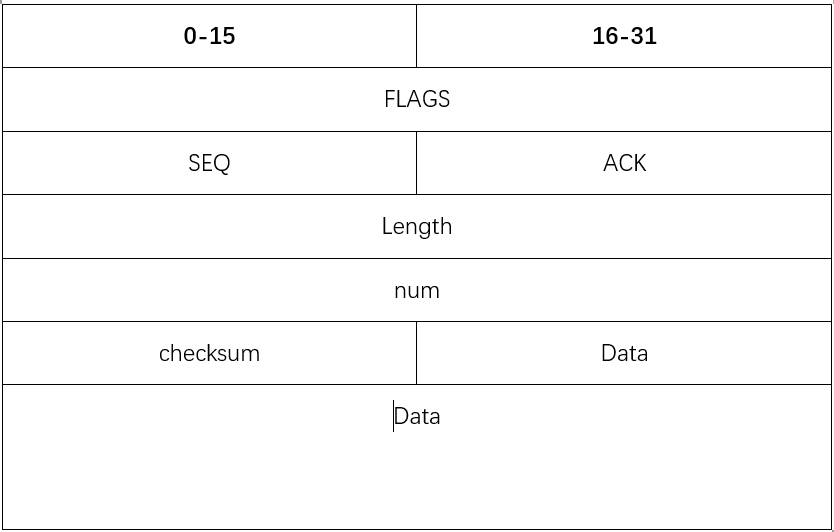
\includegraphics[scale=0.6]{计网1.png}
    \label{fig:1}
\end{figure}
\begin{lstlisting}[title=报文格式,frame=trbl,language={C++}]
struct message
{
#pragma pack(1)
    u_long flag{};
    u_short seq{};//序列号
    u_short ack{};//确认号
    u_long len{};//数据部分长度
    u_long num{}; //发送的消息包含几个包
    u_short checksum{};//校验和
    char data[8192]{};//数据长度
#pragma pack()
}
\end{lstlisting}
flags为我们所设计的伪首部,其中包含了SYN、FIN、START、END位,分别表示包的基本信息,还有一个EXIST位,表示包不为空(由于我们使用非阻塞模式,需要有此设置)。这五位,分别由flags的第一位、第二位、第四位、第八位、第十六位表示,其他位由0补齐。\par
我们的DATA为所传输的图片或文字的部分,本次实验为了减少调试和文件传输的时间,将大小调整为8192。
\subsubsection{建立连接}
\textbf{与第一次实验相同。}建立连接的过程,仿照了三次握手的过程,客户端发送带有标识SYN的消息x,接收到对方对消息x的确认消息ACK。由客户端发出第一次握手的请求,然后服务器发回第二次握手,唯一的区别是我这里客户端发出的第三次握手并不会真的被服务器收到,原因很简单,因为我们是单向传输的。
下面是大致的流程图:
\begin{figure}[H]
    \centering
    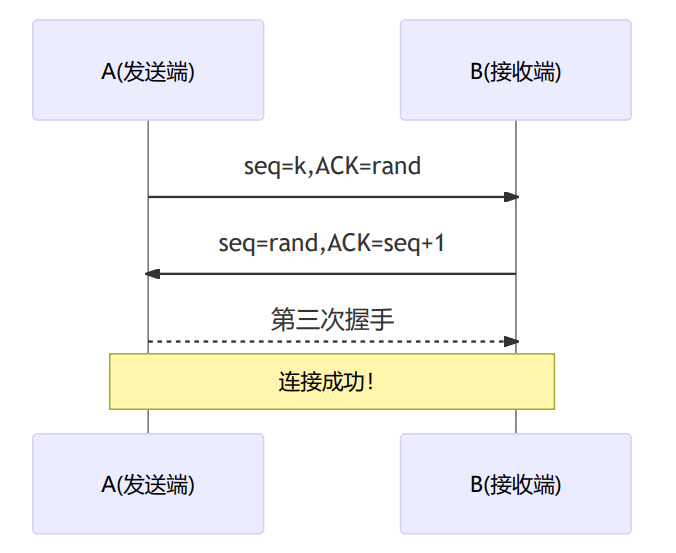
\includegraphics[scale=0.6]{计网2.png}
    \label{fig:2}
\end{figure}
具体代码实现如下所示:
\begin{lstlisting}[title=客户端,frame=trbl,language={C++}]
int beginconnect()
{
    SetColor(0,12);
    cout << "开始连接!发送第一次握手!" << endl;
    message recvMsg, sendMsg;
    sendMsg.setSYN();
    sendMsg.seq = 88;
    sendmessage(sendMsg);
    int start = clock();
    int end;
    while (true)
    {
        recvMsg = recvmessage();
        if (!recvMsg.isEXT())
        {
            end = clock();
            if (end - start > 2000) {
                SetColor(0,12);
                cout << "连接超时,请确认网络通畅和服务端启动无误后再运行本程序!" << endl;
                break;
            }
            continue;
        }
        if (recvMsg.isACK() && recvMsg.isSYN()&& recvMsg.ack == sendMsg.seq + 1) {
            SetColor(14,0);
            cout << "收到第二次握手!" << endl;
            break;
        }
    }
    sendMsg.setACK();
    sendMsg.seq = 89;
    sendMsg.ack = recvMsg.seq + 1;
    SetColor(14,0);
    cout << "发送第三次握手的数据包" << endl;
    sendmessage(sendMsg);
    return 0;
}
\end{lstlisting}

\begin{lstlisting}[title=服务器,frame=trbl,language={C++}]
int WaitConnect()
{
    SetColor(14,0);
    cout << "服务器等待连接" << endl;
    message recvMsg, sendMsg;
    while (true)
    {
        recvMsg = recvmessage();
        if (recvMsg.isSYN())
        {
            SetColor(14,0);
            cout << "收到第一次握手成功!" << endl;
            break;
        }
    }
    sendMsg.setSYN();
    sendMsg.setACK();
    sendMsg.ack = recvMsg.seq + 1;   // 将要发送确认包的ack设为收到包的seq+1
    sendMsg.setSYN();
    SetColor(14,0);
    cout << "发送第二次握手信息!" << endl;
    sendmessage(sendMsg);
    SetColor(14,0);
    cout << "接收到确认连接,连接成功" << endl;
    int iMode = 0; //1:非阻塞,0:阻塞
    ioctlsocket(Server, FIONBIO, (u_long FAR*) & iMode);//非阻塞设置
    return 0;
}
\end{lstlisting}
\subsubsection{断开连接}
\textbf{与第一次实验相同。}断开连接采用的是两次挥手,由客户端开始发出第一次挥手,服务器收到挥手后返回第二次挥手,然后双方程序结束运行。

具体代码实现如下所示:
\begin{lstlisting}[title=客户端,frame=trbl,language={C++}]
int closeconnect() {  // 断开连接
    message recvMsg, sendMsg;
    sendMsg.setFIN();
    sendMsg.seq = 65534;//此处是u_short的表示范围的最大值-1,而我们收到的将会再加一,那么已经到了u_short的最大值了,就自然结束了。
    sendmessage(sendMsg);
    cout << "发送出去第一次挥手!" << endl;
    int count = 0;
    while (true) {
        Sleep(100);
        if (count >= 50) {
            SetColor(0,12);
            cout << "等待时间太长,退出连接" << endl;
            return closeconnect();
        }
        recvMsg = recvmessage();
        if (!recvMsg.isEXT()) {
            continue;
        }
        if (recvMsg.isACK() && recvMsg.ack == sendMsg.seq + 1) {
            break;
        }
        count++;
    }
    SetColor(0,12);
    cout << "接收到确认连接,断开连接成功" << endl << endl;
    return 0;
}
\end{lstlisting}
客户端此处的第一次挥手有一个小的设计是把seq设置为u\_short的表示范围的最大值-1,而我们收到的将会再加一,那么已经到了u\_short的最大值了,就自然结束了。
\begin{lstlisting}[title=服务器,frame=trbl,language={C++}]
int closeconnect(message msg){
    message sendMsg;
    sendMsg.setACK();
    sendMsg.ack = msg.seq + 1;
    sendmessage(sendMsg);
    SetColor(14,0);
    cout<<"已经收到客户端发过来的挥手请求,并且发送了第二次挥手,服务器将结束运行!再见!"<<endl;
    return 0;
}
\end{lstlisting}
\subsubsection{差错检测}
\textbf{与第一次实验相同。}主要是校验和计算的函数,这个函数修改自老师课上所给出的方法,也就是说,如果校验和为0的话,我们的包就是正确的。具体代码如下:
\begin{lstlisting}[title=校验和计算,frame=trbl,language={C++}]
void setchecksum(){
    int sum = 0;
    u_char* temp = (u_char*)this;
    for (int i = 0; i < 8; i++)
    {
        sum += (temp[i<<1] << 8) + temp[i<<1|1];
        while (sum > 0xffff)
        {
            int t = sum >> 16;  
            sum += t;
        }
    }
    checksum = ~(u_short)sum;  
}
\end{lstlisting}
然后以此为基础进行差错检验
\begin{lstlisting}[title=差错检验,frame=trbl,language={C++}]
bool corrupt(){
        // 包是否损坏
        int sum = 0;
        u_char* temp = (u_char*)this;
        for (int i = 0; i < 8; i++)
        {
            sum += (temp[i<<1] << 8) + temp[i<<1|1];
            while (sum >= 0x10000)
            {//溢出
                int t = sum >> 16;//计算方法与设置校验和相同
                sum += t;
            }
        }
        //把计算出来的校验和和报文中该字段的值相加,如果等于0xffff,则校验成功
        if (checksum + (u_short)sum == 65535)
            return false;
        return true;
    }
\end{lstlisting}
\subsection{文件读写}
首先我们需要打开文件,这一步做出了一定的修改,先把文件整个读到内存之中,然后再复制到缓冲区之中。具体代码如下所示:
\begin{lstlisting}[title=打开文件,frame=trbl,language={C++}]
int openFile() {
    SetColor(0,10);
    cout << "请输入要发送的文件名:";
    memset(filepath, 0, 20);
    string temp;
    cin >> temp;
    if (temp == "FINISH") {
        return closeconnect();
    } else {
        strcpy(filepath, temp.c_str());
        in.open(filepath, ifstream::in | ios::binary);// 以二进制方式打开文件
        in.seekg(0, std::ios_base::end);  // 将文件流指针定位到流的末尾
        filelen = in.tellg();
        messagenum = filelen / 8192 + 1;
        SetColor(0,6);
        lastlen = filelen - (messagenum - 1) * 8192;
        cout << "文件大小为" << filelen << "Bytes,总共有" << messagenum << "个数据包" << endl;
        in.seekg(0, std::ios_base::beg);  // 将文件流指针定位到流的开始
        int index = 0, len = 0;
        // 将文件读入缓冲区
        char t = in.get();
        while (in) {
            buffer[index][len] = t;
            len++;
            if (len == 8192) {
                len = 0;
                index++;
            }
            t = in.get();
        }
        in.close();
        return 1;
    }
    else{
        SetColor(12,0);
        cout<<"文件不存在,请重新输入您要传输的文件名!"<<endl;
        return openFile();
    }
}
}
\end{lstlisting}
\section{拥塞控制}
\subsection{状态转换图}
\textbf{本次实验采用RENO算法},状态图大致如下所示:
\begin{figure}[H]
    \centering
    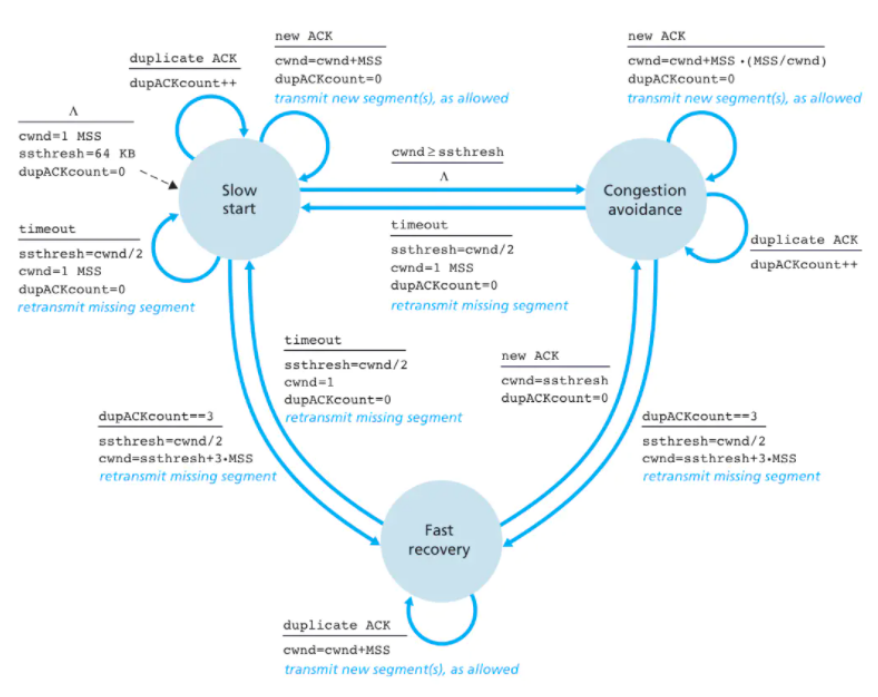
\includegraphics[scale=0.6]{cn3.png}
    \label{fig:3}
\end{figure}
\subsection{拥塞控制流程}
\subsubsection{慢启动}
\begin{enumerate}
  \item 初始时窗口大小 (cwnd) 为 1,慢启动阈值 (ssthresh) 设为 32。
  \item 每当传输的报文段首次被确认,窗口大小加 1,此时窗口大小以指数增长。
  \item 如果发生超时的丢包事件(拥塞),将慢启动阈值设为当前窗口大小的一半,并将窗口
  \item 大小设为 1,重新开始慢启动。
  \item 当窗口大小不小于慢启动阈值时,进入拥塞避免阶段。
  \item 收到冗余 ACK 时,记录数量,连续收到三次冗余 ACK 时,进入快速重传阶段。
\end{enumerate}
\subsubsection{拥塞避免}
\begin{enumerate}
  \item 拥塞避免时,更加谨慎地增加窗口大小。每收到新的 ACK,窗口大小增长 1,此时以线性增长。
  \item 收到新的 ACK,将冗余 ACK 数量置 0。
  \item 收到冗余 ACK 时,记录数量,连续收到三次冗余 ACK 时,进入快速重传阶段。
  \item 发生超时的丢包事件,重新开始慢启动。
\end{enumerate}
\subsubsection{快速恢复}
\begin{enumerate}
  \item 每收到一个冗余 ACK,窗口大小加 1,直到窗口大小大于阈值,进入拥塞避免阶段。
  \item 收到新的 ACK,进入拥塞避免阶段。
  \item  发生超时的丢包事件,重新开始慢启动。
\end{enumerate}

\subsection{多线程编程}
\textbf{在3-2已经写好多线程的基础上,只需要添加窗口控制的部分即可。}
主要分析有发送和接收线程。同时,实现选择重传,每个要发送的数据包需要一个单独的线程,用于判断数据包是否丢失或超时。
并且需要判断当前的窗口大小。
\begin{lstlisting}[title=发送线程函数,frame=trbl,language={C++}]
int sendthread() {
    bool sending = true;
    message msg;
    while (sending) {
        sendtop = sendbase + cwnd;
        for (int i = sendbase; i <=min(sendtop, messagenum - 1); i++) {
            if (state[i] == 0) {
                state[i] = -1;
                msg.seq = i;
                sendOneMsg(msg,i);
                if (i == messagenum - 1) {
                    sending = false;
                }
            }
        }
    }
    ExitThread(TRUE);
}
\end{lstlisting}
接下来是接收线程,\textbf{接收线程主要实现的是RENO算法之中对于窗口大小变化的部分,这是整个lab3-3的精华所在}:
\begin{lstlisting}
int recvthread() {
    while(1) {
        message msg = recvmessage();
        while (!msg.isEXT()) {
            continue;
        }
        if (msg.isACK()) {
            time_t now_time = time(NULL);
            tm *t_tm = localtime(&now_time);
            cout << "收到ack为" << msg.ack << "的数据包" << endl;
            cout << asctime(t_tm) << endl;
            state[msg.ack] = 1;
            cout << endl;
            if (state[msg.ack] == 1) {
                if (flag != 2) {
                    redundancy++;
                } else {
                    cout << "指数增长" << endl;
                    cwnd += 1;
                }
                cout << "收到第" << redundancy << "个冗余数据包" << endl;
                if (redundancy >= 3) {
                    cout << "开始快速重传" << endl;
                    flag = 2;
                    ssthresh = cwnd / 2;
                    cwnd = ssthresh + 3;
                }
                return 1;
            } else {
                if (flag == 1) {
                    redundancy = 0;
                }
                if (flag == 2) {
                    flag = 1;
                    redundancy = 0;
                }
                state[msg.ack] = 1;
                cout<<"len="<<msg.len<<", checksum="<<msg.corrupt()<<", flag="<<msg.flag<<", seq="<<msg.seq<<endl;
                if (cwnd >= ssthresh) {
                    flag = 1;
                    cout << "线性增长" << endl;
                    cwnd += 1 / cwnd;

                }
                else {
                    cout << "指数增长" << endl;
                    cwnd += 1;
                }
                if (msg.ack == messagenum - 1) {
                    ExitThread(TRUE);
                }
            }
        }
    }
}
\end{lstlisting}
\subsubsection{超时重传}
关于超时机制,仍然采取了RDT3.0的设计,对于窗口内的任何单个包,我们都要设置一个计时器,如果这个包丢包、传输错误、超时等任何原因导致一旦超过我们设计的限定时间,就要进行重发机制。并且会在屏幕输出“传输超时”。
\begin{lstlisting}[title=超时重传,frame=trbl,language={C++}]
int sendOneMsg(message msg,int num) {
    if (num != messagenum - 1) {
        memcpy(msg.data, buffer[num], 8192);
        msg.len = 8192;
    }
    else {
        memcpy(msg.data, buffer[num], lastlen);
        msg.len = lastlen;
    }
    msg.seq = num;
    sendmessage(msg);

    clock_t start = clock();
    while (1) {
        clock_t end = clock();
        if (end - start > TIMEOUT) {
            flag = 0;   // 超时,回到慢启动
            redundancy = 0;
            if (isFINISH) {return 0;}
            cout << "传输超时" << endl;
            sendmessage(msg);
            start = clock();
            //lab3-3
            ssthresh = cwnd / 2;
            cwnd = 1;
        }
        if (state[num] == 1) {
            cout<<"len="<<msg.len<<", checksum="<<msg.checksum<<", flag="<<msg.flag<<", seq="<<msg.seq<<endl;
            return 1;
        }
    }
    return 1;
}
\end{lstlisting}
\subsubsection{文件传输流程}
大致内容是在开启接收和发送的线程之后,执行发送和接收的功能。其中,关于窗口滑动的功能,写了一个选择语句,即当窗口上沿已经到了最后一个数据包的时候,就不再增长了。
\begin{lstlisting}[title=客户端发送文件,frame=trbl,language={C++}]
    cout << "开始发送文件内容!" << endl;
    sendbase = 0;
    cwnd = 0;
    redundancy = 0;
    isEnd = false;
    bool sending = true;
    timestart = clock();
    int n = 0;
    // 创建一个接收线程
    thread recvThr(recvthread);
    if (recvThr.joinable()) {
        recvThr.detach();
    }
    else {
        cout << "create recvthread failed!" << endl;
        return -1;
    }
    // 创建一个发送线程
    cout << "开始发送文件" << endl;
    thread sendThr(sendthread);
    if (sendThr.joinable()) {
        sendThr.detach();
    }
    else {
        cout << "create sendthread failed!" << endl;
        return -1;
    }

    while (sending) {
        while (status[sendbase] == 1) {
            redundancy = 0;
            // 收到当前滑动窗口底的数据包ack
            cout << "滑动窗口前移" << endl;
            if (sendbase == packetnum - 1) { // 除最后一个包都接收到ack
                sending = false;
                isEnd = true;
                break;
            }
            sendbase++;
            cout << "sendbase:" << sendbase << "sendtop:" << sendtop << "WINDOW_SIZE:"<<sendtop-sendbase<<endl;
        }
    }
    cout << "成功发送文件!" << endl;
    timeend = clock();
    double endtime = (double)(timeend - timestart) / CLOCKS_PER_SEC;
    cout << "传输总时间" << endtime << "s" << endl;
    cout << "吞吐率" << (double)(packetnum) * sizeof(packet) * 8 / endtime  / 8192 << "kbps" << endl;
\end{lstlisting}

\begin{lstlisting}[title=服务器接收文件,frame=trbl,language={C++}]
int recvMsg() {
    recvbase = 0;
    recvtop =((messagenum <= windowSize)?(messagenum - 1):( windowSize - 1));
    cout << "正在接收文件" << endl;
    thread recvThr(recvThread);
    recvThr.detach();
    while (recving) {
        while (state[recvbase] == 1) {
            cout << "滑动窗口前移一位" << endl;
            if (recvbase == messagenum - 1) {
                recving = false;
                break;
            }
            recvbase=((recvbase==(messagenum-1))?recvbase:recvbase+1);
            recvtop=((recvtop<(messagenum-1))?recvtop+1:recvtop);
            cout << "现在窗口底部是:" << recvbase << ", 现在窗口顶部是:" << recvtop << endl;
        }
    }
    isFINISH = true;
    cout << "接收文件完成!" << endl;
    int i;
    for (i = 0; i < messagenum - 1; i++) {
        out.write(buffer[i], 8192);
    }
    out.write(buffer[i], lastlen);
    out.close();
    out.clear();
    recvbase = 0;
    recvtop = windowSize - 1;
    cout << "写文件完成" << endl;
    return getFileName();
}
\end{lstlisting}
\subsubsection{丢包设计}
由于所提供的router.exe不能使用,因此我自行设置了一个丢包的函数,原理是设置随机数,然后用随机数mod100,以此设计丢包率,代码如下所示:
\begin{lstlisting}[title=丢包函数,frame=trbl,language={C++}]
int judgeRand(){
    int s=rand()%100;
    if(s<10){return 0;}
    else{return 1;}
}
\end{lstlisting}
\begin{lstlisting}[title=发送函数,frame=trbl,language={C++}]
void sendmessage(message msg) {
    msg.setEXT();
    msg.setchecksum();
    if(judgeRand()==1){
    if (sendto(Client, (char*)&msg, BUFFER, 0, (SOCKADDR*)&serveraddr, sizeof(SOCKADDR)) == (SOCKET_ERROR)) {
        SetColor(0,12);
        cout << "发送错误了!!" << endl;
    }}
}
\end{lstlisting}
\subsection{结果展示}
首先是建立连接的过程:
\begin{figure}[H]
    \centering
    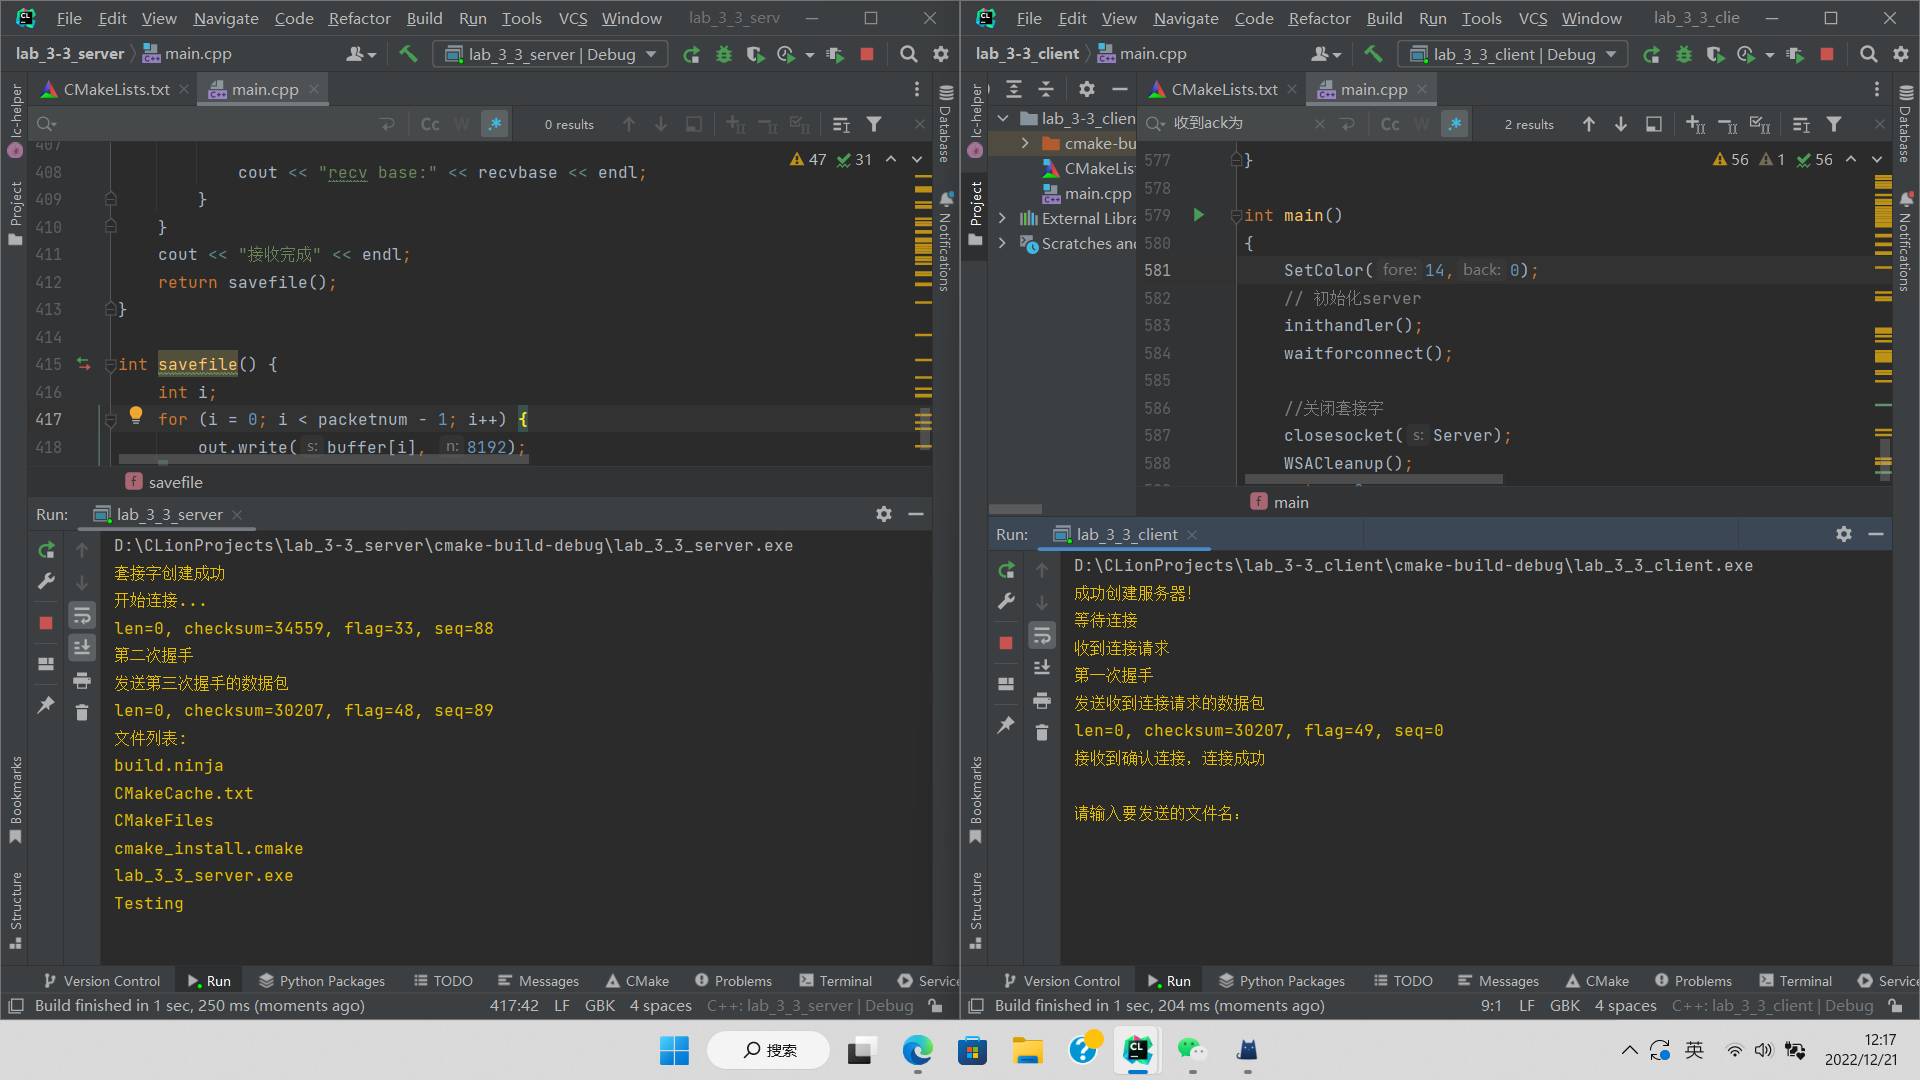
\includegraphics[scale=0.4]{GW1.png}
    \label{fig:6}
\end{figure}
这里我增加了一个扫描文件夹的功能,可以看到在发送之前我们是没有1.jpg这个文件的。
接下来是发送文件的过程和最后断开连接的过程:
\begin{figure}[H]
    \centering
    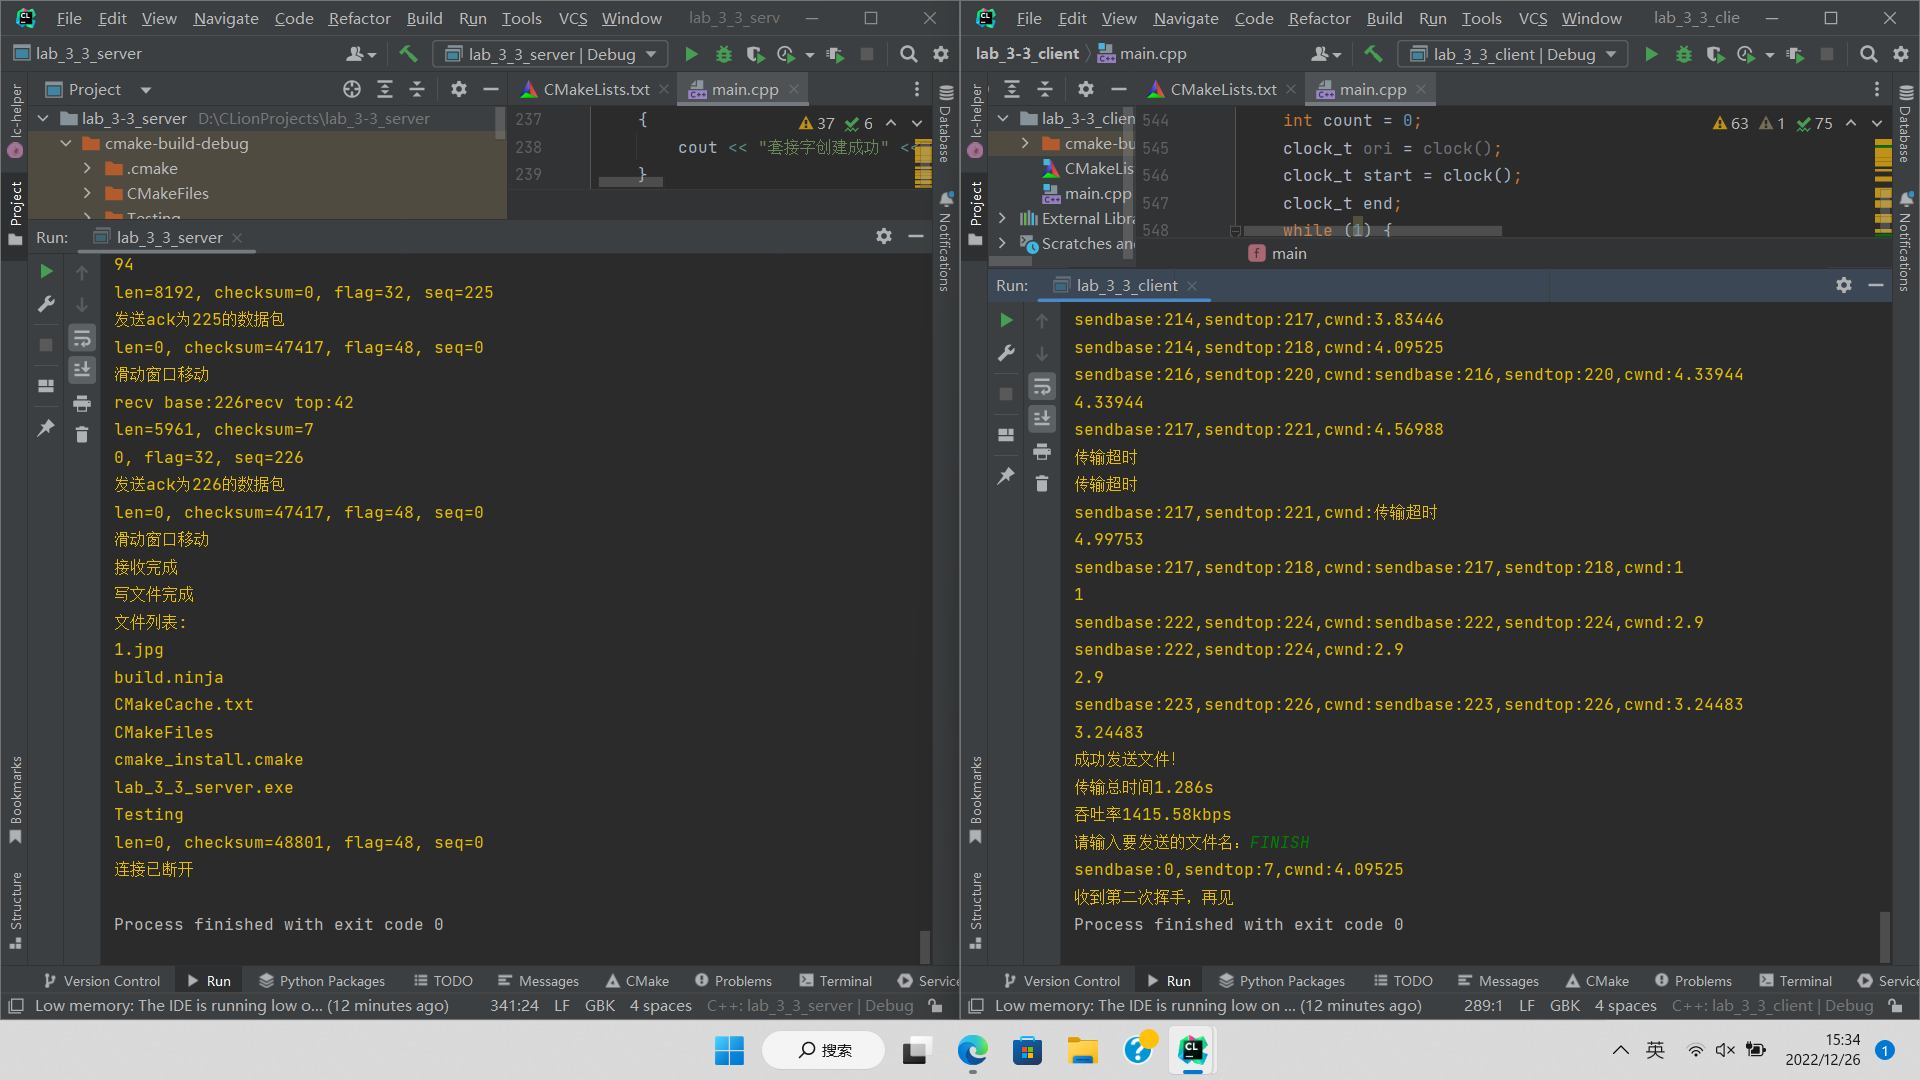
\includegraphics[scale=0.4]{GW2.png}
    \label{fig:7}
\end{figure}
可以看到文件发送成功。同时,我们看到文件夹之下出现了1.jpg这个文件。这证明我们发送成功了。可以看到断开连接也是成功的。

然后展示一些窗口变化的部分,这里为了防止IO资源竞争,只打印了窗口部分日志用来说明。

首先在一开始是慢启动阶段,可以看到一开始拥塞控制处于慢启动阶段,每次收到ACK消息窗口都增加1。直到cwnd> ssthresh,程序进入拥塞避免阶段,窗口大小增长减慢。
\begin{figure}[H]
    \centering
    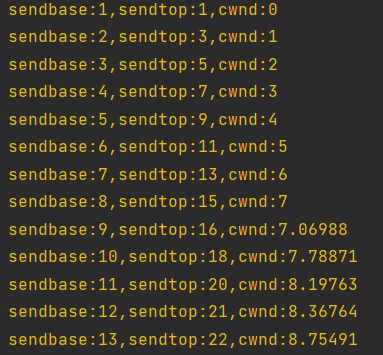
\includegraphics[scale=0.5]{GW3.png}
    \label{fig:7}
\end{figure}
这不是拥塞避免阶段了,这里是我们人为丢包的程序起了作用,发送端会进入快速恢复阶段,此时ssthresh=cwnd/2, cwnd=ssthresh+3。
\begin{figure}[H]
    \centering
    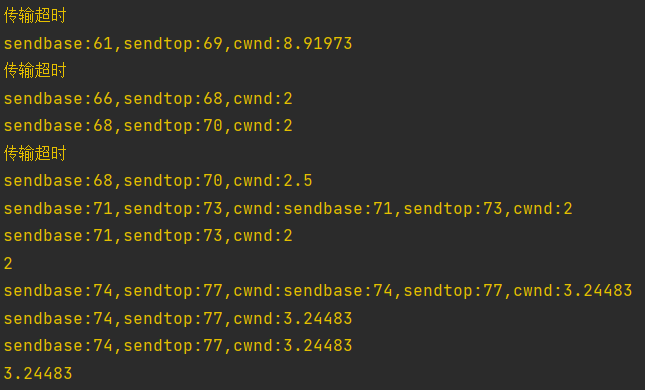
\includegraphics[scale=0.4]{GW4.png}
    \label{fig:7}
\end{figure}
最后我们又挑选了一个拥塞控制从快速恢复阶段进入慢启动阶段的日志进行分析。
\begin{figure}[H]
    \centering
    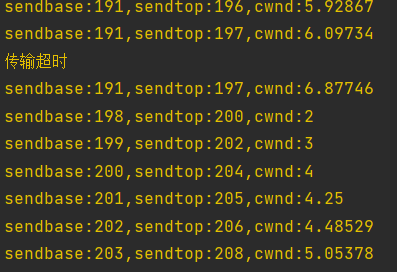
\includegraphics[scale=0.5]{GW5.png}
    \label{fig:7}
\end{figure}
\section{总结与一些问题}
本次实验较为成功实现了拥塞控制功能,很有收获。由于随机数函数生成的随机数较为接近,容易造成程序出现问题,因此部分结果展示的内容进行了多次实验,并不是同一次的日志。
\end{document}